\section{Założenia badawcze i konfiguracja eksperymentów}
\label{sec:zalozenia-badawcze-i-konfiguracja-eksperymentow}

Eksperymenty zaplanowano jako porównanie jakości transkrypcji pisma odręcznego. Każdy model otrzymywał obraz pojedynczej linii tekstu i zwracał rozpoznany tekst. Wynik porównywano z transkrypcją referencyjną.

Modele nie klasyfikowały dysgrafii. Informacja o dysgrafii była metadanym opisującym próbkę. Wykorzystano ją dopiero podczas analizy wyników, aby sprawdzić, czy jakość rozpoznawania różni się między grupami.

W eksperymentach użyto trzech rozwiązań: Kraken, TrOCR oraz Qwen3-VL. Dla każdego rozwiązania przygotowano możliwie podobny schemat pracy:

\begin{itemize}
    \item przygotowanie obrazu linii tekstu,
    \item uruchomienie inferencji,
    \item zapis predykcji modelu,
    \item porównanie predykcji z ground truth,
    \item obliczenie metryk jakości,
    \item analiza wyników w podziale na zbiory i grupy trudności.
\end{itemize}

\subsection{Wykorzystane dane}
\label{subsec:wykorzystane-dane-eksperymenty}

W badaniach wykorzystano trzy zbiory danych. Głównym zbiorem był własny dataset polskiego pisma odręcznego. Zawiera on 2313 zweryfikowanych obrazów linii pochodzących z 320 formularzy. Próbki opisano metadanymi dotyczącymi płci, roku urodzenia i deklarowanych trudności w pisaniu.

Drugim zbiorem był malezyjski dataset pisma dzieci w wieku szkolnym. Oryginalne dane zawierały grupy LPD oraz PD. Na potrzeby tej pracy przygotowano wersję liniową zbioru. Po ręcznej segmentacji i opisie danych uzyskano 488 obrazów linii z transkrypcjami.

Trzecim zbiorem był IAM. Wykorzystano go jako zbiór kontrolny. Służył do sprawdzenia, czy przygotowany kod inferencji i ewaluacji działa poprawnie także na znanym zbiorze HTR spoza głównych danych badawczych.

\begin{table}[H]
    \centering
    \caption{Zbiory danych wykorzystane w eksperymentach.}
    \label{tab:zbiory-danych-eksperymenty}
    \begin{tabularx}{\textwidth}{lXl}
        \hline
        Zbiór & Zastosowanie & Język \\
        \hline
        Własny zbiór formularzy & Główny zbiór badawczy. Analiza pisma bez trudności, pisma dysgraficznego i innych trudności. & polski \\
        Malaysian dataset & Zewnętrzny zbiór porównawczy z grupami LPD i PD. & malajski \\
        IAM & Zbiór kontrolny do sprawdzenia procedur inferencji i ewaluacji. & angielski \\
        \hline
    \end{tabularx}
\end{table}

\subsection{Przygotowanie danych do eksperymentów}
\label{subsec:przygotowanie-danych-do-eksperymentow}

Wszystkie eksperymenty prowadzono na poziomie pojedynczej linii tekstu. Dlatego każdy zbiór sprowadzono do wspólnej postaci: obraz linii oraz odpowiadający mu ground truth.

Własny zbiór pochodził z formularzy papierowych. Formularze miały stały układ i znaczniki w rogach strony. Na tej podstawie prostowano obraz formularza i wycinano linie z pismem. Następnie sprawdzano wyniki w programie walidacyjnym. W programie poprawiano transkrypcje, metadane i status próbki.

\begin{figure}[H]
    \centering
    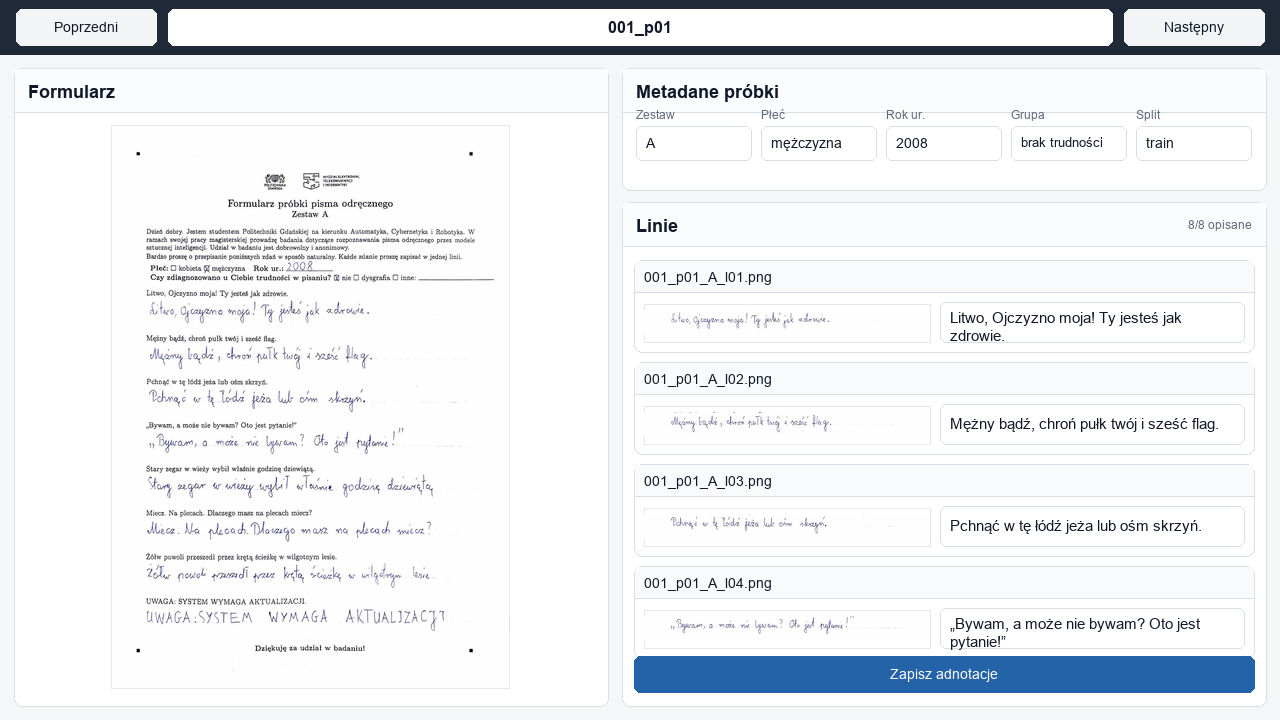
\includegraphics[width=0.95\textwidth]{Formularze/processed_320_check/stats_thesis/figures/panel_walidacji_gt_clean.png}
    \caption{Panel używany do walidacji własnego zbioru danych. Program pozwalał porównać obraz linii z wpisem w pliku CSV i poprawić ground truth.}
    \label{fig:panel-walidacji-wlasny-zbior}
\end{figure}

W zbiorze malezyjskim nie było takiego samego szablonu formularza. Linie tekstu wycinano więc ręcznie. Każdej linii przypisano transkrypcję. Do kontroli danych użyto podobnego programu pomocniczego.

\begin{figure}[H]
    \centering
    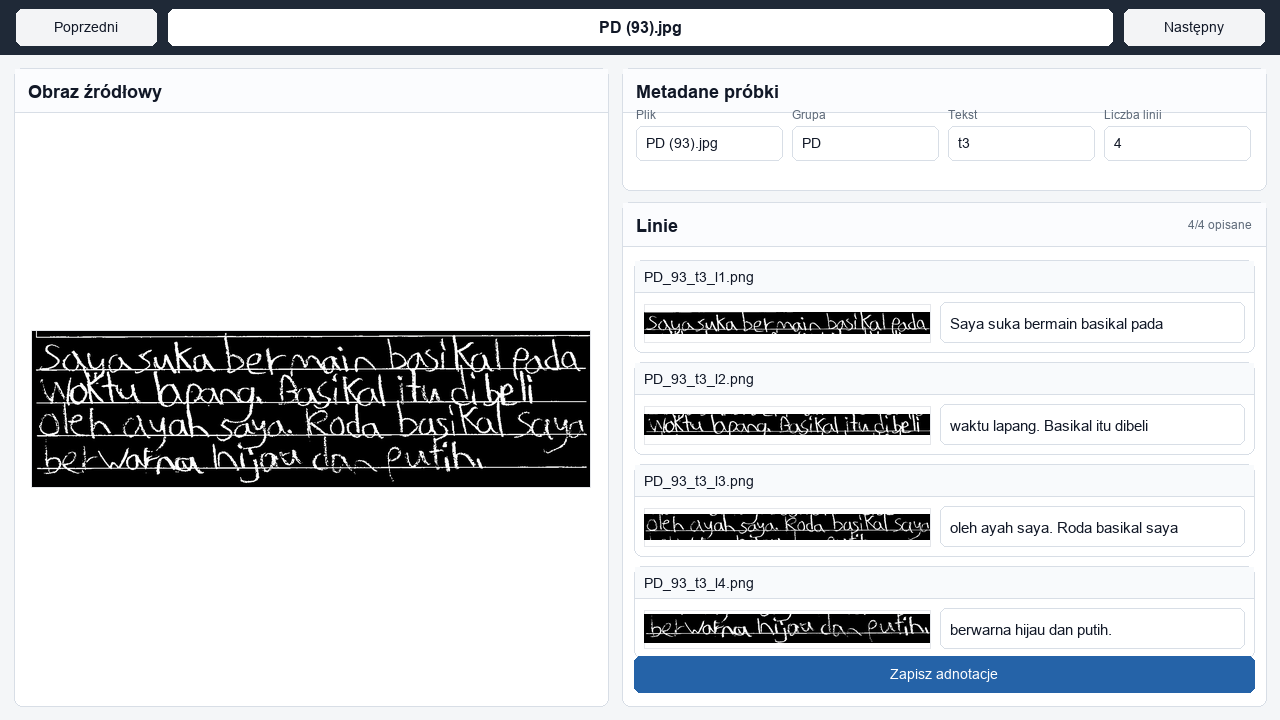
\includegraphics[width=0.95\textwidth]{Formularze/processed_320_check/stats_thesis/figures/malaysian_labeling_program.png}
    \caption{Program pomocniczy używany podczas ręcznej segmentacji i opisu linii w zbiorze malezyjskim.}
    \label{fig:panel-walidacji-malaysian}
\end{figure}

Ground truth zapisywano zgodnie z widocznym tekstem. Nie poprawiano go automatycznie do wersji językowo poprawnej ani do tekstu wzorcowego z formularza. Jeśli zapis był niejednoznaczny, próbkę oznaczano jako niepewną albo wykluczano z finalnego eksportu.

Dane zapisano w kilku formatach. Podstawowym formatem były obrazy linii oraz manifesty CSV. Dla TrOCR przygotowano strukturę zgodną z treningiem modeli Hugging Face. Dla Qwen3-VL przygotowano manifesty z obrazami i tekstem referencyjnym. Dla Krakena przygotowano dane w formacie PAGE XML.

\subsection{Podział danych}
\label{subsec:podzial-danych-eksperymenty}

Własny zbiór podzielono na część treningową, walidacyjną i testową. Podział wykonano na poziomie uczestnika. Linie tej samej osoby nie trafiały więc jednocześnie do treningu i testu.

\begin{table}[H]
    \centering
    \caption{Podział własnego zbioru na części eksperymentalne.}
    \label{tab:podzial-wlasnego-zbioru-eksperymenty}
    \begin{tabular}{lr}
        \hline
        Część zbioru & Liczba obrazów linii \\
        \hline
        Treningowa & 1844 \\
        Walidacyjna & 228 \\
        Testowa & 241 \\
        \hline
        Razem & 2313 \\
        \hline
    \end{tabular}
\end{table}

Zbiór testowy traktowano jako część końcowej ewaluacji. Nie używano go do treningu ani do doboru parametrów. Zbiór walidacyjny służył do kontroli przebiegu dostrajania.

\subsection{Scenariusze eksperymentalne}
\label{subsec:scenariusze-eksperymentalne}

Pierwszym scenariuszem była inferencja zero-shot. W tym wariancie uruchamiano gotowe modele bez uczenia ich na analizowanych zbiorach. Ten etap dał punkt odniesienia dla późniejszych eksperymentów.

Drugim scenariuszem był fine tuning. W tym wariancie dostrajano model na danych treningowych, kontrolowano wyniki na danych walidacyjnych i raportowano wynik na danych testowych.

\begin{table}[H]
    \centering
    \caption{Główne scenariusze eksperymentalne.}
    \label{tab:scenariusze-eksperymentalne}
    \begin{tabularx}{\textwidth}{lX}
        \hline
        Scenariusz & Sposób wykonania \\
        \hline
        Zero-shot & Uruchomienie gotowego modelu na obrazach linii bez dodatkowego treningu. \\
        Fine tuning standardowy & Dostrojenie modelu na części treningowej i ocena na zbiorze testowym. \\
        Fine tuning z oversamplingiem & Powielenie istniejących próbek dysgraficznych w treningu. Nie tworzono syntetycznych obrazów. \\
        Mixed-domain & Uczenie z użyciem danych pochodzących z więcej niż jednego zbioru. \\
        \hline
    \end{tabularx}
\end{table}

W przypadku Qwen3-VL użyto promptu z poleceniem przepisania tekstu z obrazu. W części dostrajania zastosowano LoRA. W przypadku TrOCR wykonano fine tuning na obrazach linii i odpowiadających im transkrypcjach. W przypadku Krakena dane przygotowano jako PAGE XML i uruchomiono trening poleceniem \texttt{ketos train}.

Wariant z oversamplingiem miał sprawdzić, czy zwiększenie udziału próbek dysgraficznych w treningu poprawia wyniki dla tej grupy. Oversampling polegał wyłącznie na powieleniu istniejących próbek. Nie generowano nowych obrazów pisma.

\subsection{Środowisko implementacyjne}
\label{subsec:srodowisko-implementacyjne}

Prace wykonano w dwóch środowiskach. Lokalnie używano systemu Windows, PowerShella, Pythona, wirtualnych środowisk Python i notebooków Jupyter. To środowisko służyło głównie do przygotowania danych, walidacji datasetów, organizacji manifestów CSV, generowania wykresów i tabel oraz eksperymentów z Krakenem.

Modele wymagające większej ilości pamięci GPU uruchamiano w Google Colab. Dotyczyło to przede wszystkim fine tuningu Qwen3-VL i TrOCR. W Colabie korzystano z CUDA, PyTorch, Hugging Face Transformers, PEFT/LoRA, \texttt{datasets} oraz \texttt{accelerate}. Checkpointy i wyniki zapisywano na Google Drive.

\begin{table}[H]
    \centering
    \caption{Podział prac między środowiska implementacyjne.}
    \label{tab:srodowiska-implementacyjne}
    \begin{tabularx}{\textwidth}{lX}
        \hline
        Środowisko & Zakres prac \\
        \hline
        Windows lokalnie & Preprocessing, walidacja danych, manifesty CSV, wykresy, tabele, część ewaluacji, Kraken. \\
        Google Colab & Fine tuning Qwen3-VL, fine tuning TrOCR, ewaluacja modeli wymagających GPU, zapis checkpointów. \\
        \hline
    \end{tabularx}
\end{table}

Do obróbki danych i wyników używano bibliotek \texttt{pandas}, \texttt{numpy}, \texttt{matplotlib}, \texttt{Pillow}, \texttt{jiwer} i \texttt{openpyxl}. Dane wejściowe przechowywano jako obrazy linii i manifesty CSV. Wyniki zapisywano jako CSV, JSON lub XLSX. Wykresy eksportowano jako PNG.

\subsection{Ewaluacja}
\label{subsec:ewaluacja-modeli}

Ewaluacja polegała na porównaniu predykcji modelu z ground truth. Nie stosowano końcowej korekty językowej. Dzięki temu wynik opisywał jakość rozpoznawania pisma, a nie skuteczność poprawiania tekstu po rozpoznaniu.

Podstawowymi metrykami były CER oraz WER. Liczono także corpus CER i corpus WER. Dodatkowo raportowano CLA, CRW, exact match rate, czas inferencji oraz zużycie pamięci tam, gdzie było to możliwe.

Wyniki analizowano dla całych zbiorów oraz w grupach. Dla własnego zbioru najważniejszy był podział na brak trudności, dysgrafię i inne trudności. Dla zbioru malezyjskiego analizowano grupy LPD i PD. Wykonano także analizę błędów na poziomie znaków i słów, ze szczególną uwagą na polskie znaki diakrytyczne, cyfry i interpunkcję.

\FloatBarrier
